% !TeX root = ../../main.tex


\section{井筒内结垢物运移及分布规律研究}
海上油井钡锶垢是由地层水与注入水（如海水）混合后，因钡（$\mathrm{Ba^{2+}}$）、锶（$\mathrm{Sr^{2+}}$）离子与硫酸根（$\mathrm{SO_4^{2-}}$）或碳酸根（$\mathrm{CO_3^{2-}}$）结合形成的难溶性无机盐（如硫酸钡、硫酸锶），在井筒、管道或设备表面沉积形成的坚硬垢层；其生成受高温高压、高矿化度及流动条件影响，易堵塞油流通道、加剧设备腐蚀，甚至因伴生放射性物质（如镭）带来安全与环保风险。
研究钡锶垢的运移规律在油井洗井中至关重要，通过明确垢颗粒的迁移和沉降特性，优化洗井工艺参数，高效清除井筒和近井地带的顽固垢层，避免二次堵塞或地层伤害，从而恢复油井产能并延长寿命；同时可预测垢的沉积风险，指导防垢措施以减少设备腐蚀和放射性污染，降低维护成本与环境危害，并为建立结垢动力学模型、开发新型洗井技术提供理论支撑，最终实现安全、经济、环保的油田开发目标。

建立两种尺寸不同的钡锶垢颗粒模型，如图\ref{fig:BaSr_particle}所示。通过调研钡锶垢的物理性质及性状，将其运移仿真参数列于表\ref{tab:basr_simulation_params}。

\begin{figure}[htbp]
    \centering
    % 子图 (a)
    \subfloat[钡锶垢实物]{%
        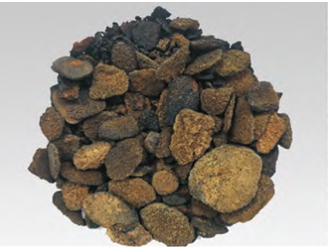
\includegraphics[width=0.48\linewidth]{figure/BaSr-sample.png}%
        \label{fig:BaSr_sample}%
    }
    \hfill
    % 子图 (b)
    \subfloat[SEM微观形貌]{%
        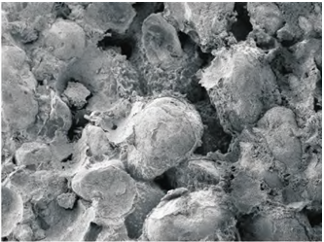
\includegraphics[width=0.48\linewidth]{figure/BaSr-SEM.png}%
        \label{fig:BaSr_SEM}%
    }
    \vspace{1em}
    % 子图 (c)
    \subfloat[垢仿真模型示意图]{%
        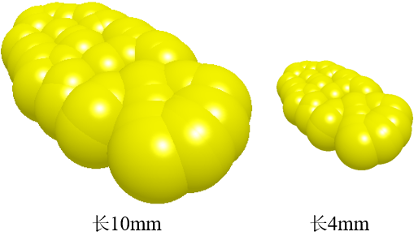
\includegraphics[width=0.5\linewidth]{figure/BaSr-model.png}%
        \label{fig:BaSr_model}%
    }
    \caption{钡锶垢颗粒及仿真模型对比}
    \label{fig:BaSr_particle}
\end{figure}

\begin{table}[htbp]
    \centering
    \caption{锁锶垢颗粒运移仿真参数}
    \label{tab:simulation_params}
    \begin{tabularx}{.9\textwidth}{CCCC}
        \toprule % 顶部粗线
        名称 & 符号 & 数值 & 单位 \\
        \midrule % 中间细线
        水平井筒长度 & $L$ & 1.5 & m \\
        井筒直径 & $D_H$ & 177.8 & mm \\
        钻杆直径 & $D_P$ & 88.9 & mm \\
        颗粒密度 & $\rho_P$ & 4336.0 & kg/m$^3$ \\
        洗井液密度 & $\rho_l$ & 1300.0 & kg/m$^3$ \\
        井斜角度 & $\theta$ & 0、45、90 & $^\circ$ \\
        洗井液入口流速 & $v_{in}$ & 0.37、0.59 & m/s \\
        洗井液粘度 & $\mu$ & 1.7 & mPa$\cdot$s \\
        沉积域距离井壁高度 & $H$ & 20.0 & mm \\
        颗粒与井壁静摩擦系数 & $\mu_s$ & 0.5 & - \\
        颗粒与井壁滑动摩擦系数 & $\mu_k$ & 0.4 & - \\
        \bottomrule % 底部粗线
    \end{tabularx}
\end{table}

\subsection{洗井液流速对钡锶垢运移规律的影响}

选取井斜$\theta = 45^\circ$，洗井液入口流速$V_{\mathrm{in}}$取$0.37\mathrm{m/s}$和$0.59\mathrm{m/s}$两种，洗井液粘度取$1.7\mathrm{mPa\cdot s}$，钡锶垢颗粒有两种尺寸，特征长度约为$10\mathrm{mm}$和$4\mathrm{mm}$。

图\ref{fig:Ba_Sr_distribution}描述的是不同洗井液流速下井筒内钡锶垢颗粒的分布情况，入口流速对钡锶垢颗粒运移效率的影响十分明显。随着洗井液流速增大，钡锶垢颗粒的运移速度逐渐增大。由于洗井液入口流速增大，产生于颗粒工厂的钡锶垢颗粒及悬浮层颗粒具有更大的轴向位移，在相同的仿真时间内，流速高时井筒内钡锶垢颗粒距离流体入口更远。
\begin{figure}[htbp]
	\centering
	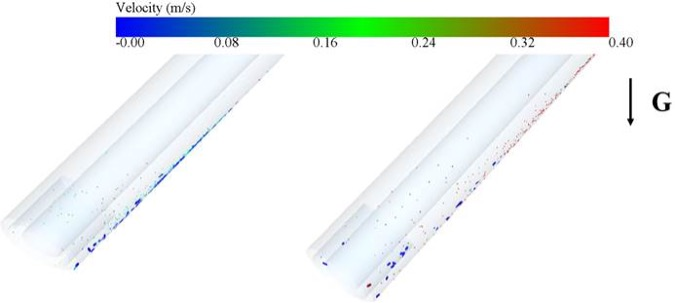
\includegraphics[width=0.7\textwidth]{figure/BaSr-distribution-Vin.jpg}
	\caption{钡锶垢颗粒在井筒中的运移}
	\label{fig:Ba_Sr_distribution}
\end{figure}

图\ref{fig:Ba_Sr_velocity_size}为钡锶垢在井筒洗井液流速$V_{\mathrm{in}}=0.37\mathrm{m/s}$和$V_{\mathrm{in}}=0.59\mathrm{m/s}$稳态后颗粒沉积域运移速度图。选取Z方向为竖直向上方向。$V_{\mathrm{in}}=0.37\mathrm{m/s}$时，大垢落到井壁上后会滑向井底，小垢在进入沉积域后会以远远低于井筒内流体的速度(约为$0.05\mathrm{m/s}$)缓慢向压力出口运移。$V_{\mathrm{in}}=0.59\mathrm{m/s}$时，大垢在进入沉积域之后Z方向速度几乎为零，少许的速度波动是由颗粒碰撞引起的，因此大垢在接触井壁后会在井壁上发生沉积现象，小垢在进入沉积域后会以低于井筒内流体的速度向压力出口运移，运移速度为$0.25\mathrm{m/s}$左右。

\begin{figure}[htbp]
	\centering
	\subfloat[$V_{\mathrm{in}}=0.37\mathrm{m/s}$]{%
	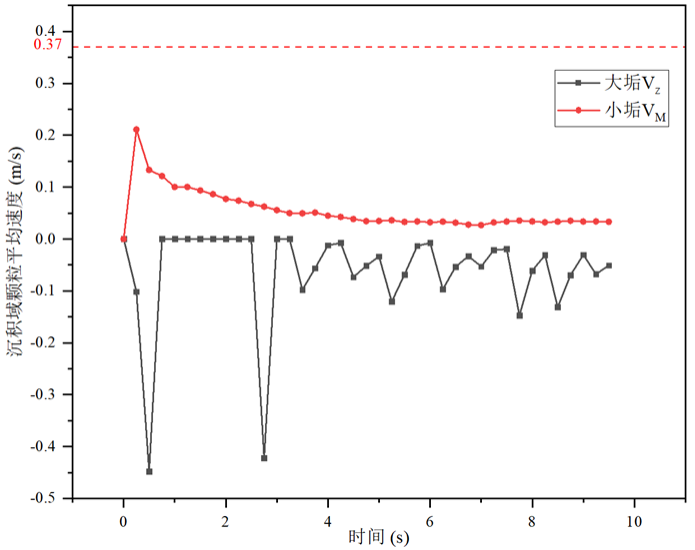
\includegraphics[width=0.48\textwidth]{figure/BaSr-mean-velocity-evolution-vin-dot37.png}
	}
	\subfloat[$V_{\mathrm{in}}=0.59\mathrm{m/s}$]{%
	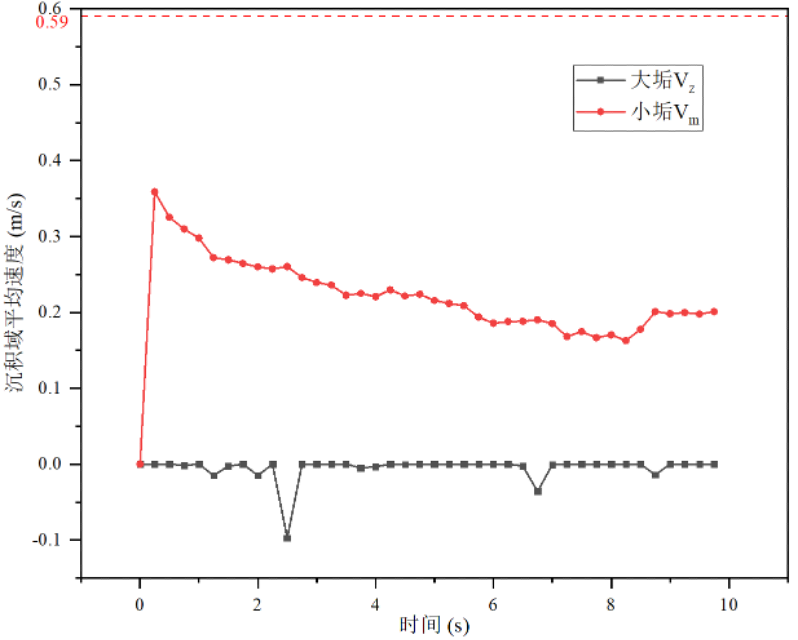
\includegraphics[width=0.48\textwidth]{figure/BaSr-mean-velocity-evolution-vin-dot59.png}
	}
	\caption{钡锶垢颗粒在沉积域运移平均速度演化}
	\label{fig:Ba_Sr_velocity_size}
\end{figure}

\subsection{井斜对钡锶垢运移规律的影响}

图\ref{fig:Ba_Sr_distribution_3angles}描述了井斜角变化时井筒内钡锶垢颗粒分布情况。$\theta=45^\circ$与$\theta=90^\circ$井斜下的钡锶垢颗粒都沉积在井底并以一定的速度向压力出口方向运移，其中$\theta=45^\circ$井筒内钡锶垢颗粒运移速度要大于$\theta=90^\circ$井筒内钡锶垢的运移速度，大颗粒钡锶垢在$\theta=45^\circ$与$\theta=90^\circ$井筒环空中均能够观察到，在直井（$\theta=0^\circ$）井筒环空中没有发现大颗粒钡锶垢，推测由于重力作用大颗粒钡锶垢产生后即下落至井底。而小颗粒钡锶垢运移速度随着井筒倾角的增大而减小，可见井筒倾角对钡锶垢运移效率有很大影响，其影响要以颗粒实际大小为准。

\begin{figure}[htbp]
	\centering
	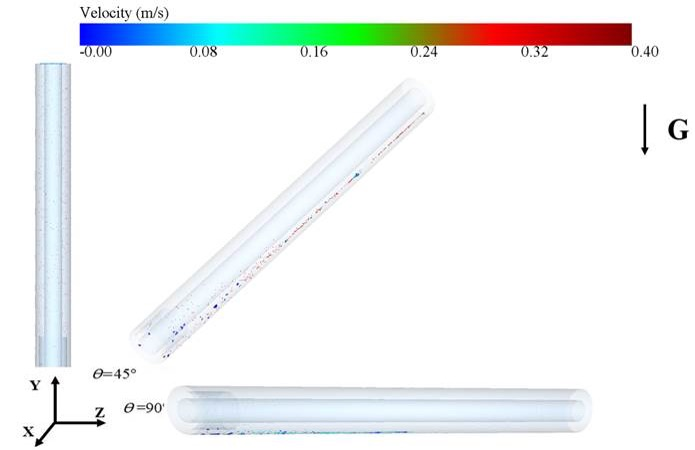
\includegraphics[width=0.7\textwidth]{figure/BaSr-distribution-3angles.jpg}
	\caption{钡锶垢颗粒在井筒中的运移}
\label{fig:Ba_Sr_distribution_3angles}
\end{figure}


图\ref{fig:Ba_Sr_velocity_3angles}(a)描述的是不同井斜下大颗粒钡锶垢井筒内运移速度变化，从图中可以看出，井斜45°与井斜90°情况下大颗粒钡锶垢因为重力影响在接触井壁后运移速度几乎为零，因此会在井壁产生沉积现场。井斜0°情况下大颗粒钡锶垢在井筒环空中运移，速度小于零说明大颗粒钡锶垢在以流体速度相反的方向运移，预测会在井底产生沉积。图\ref{fig:Ba_Sr_velocity_3angles}(b)描述的是不同井斜下小颗粒钡锶垢井筒内运移速度变化，从图中可以看出，随着井斜角的增加，钡锶垢在井筒内的运移速度逐渐减小。0°井斜下，钡锶垢在四秒左右即有颗粒到达压力出口，因为到达压力出口的钡锶垢颗粒速度减为0，随着越来越多的钡锶垢颗粒到达压力出口，其平均运移速度逐渐减小。45°与90°井斜下，钡锶垢颗粒由于重力作用在接触井筒内壁后会以一定速度向压力出口运移。由此可见，井斜可以明显影响钡锶垢颗粒的运移效率。

\begin{figure}[htbp]
	\centering
	\subfloat[$V_{\mathrm{in}}=0.37\mathrm{m/s}$]{%
	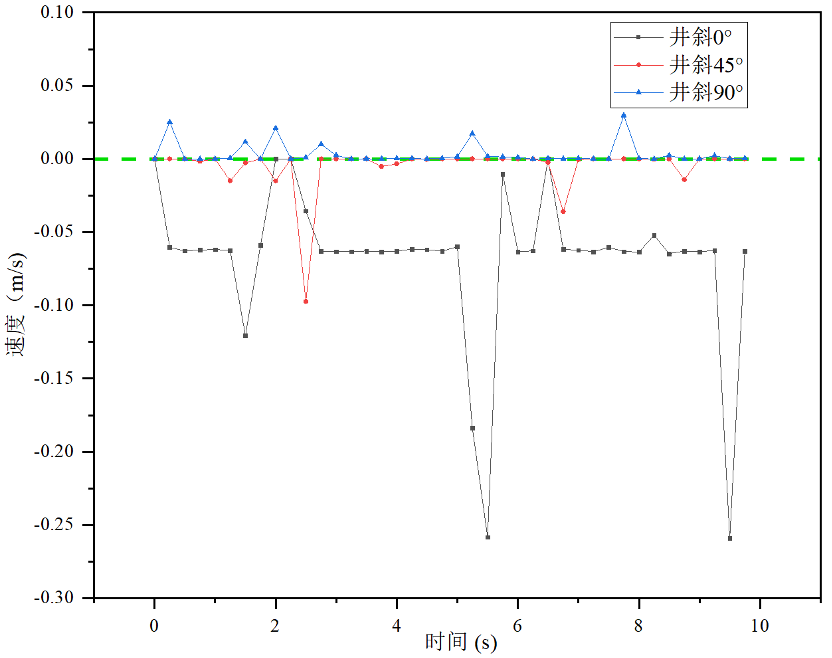
\includegraphics[width=0.48\textwidth]{figure/BaSr-mean-velocity-evolution-big-size.png}
	}
	\subfloat[$V_{\mathrm{in}}=0.59\mathrm{m/s}$]{%
	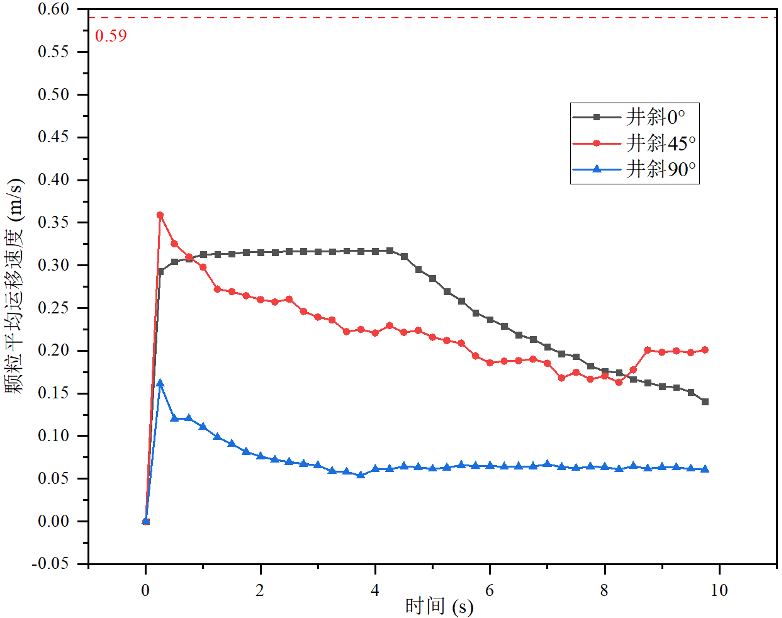
\includegraphics[width=0.48\textwidth]{figure/BaSr-mean-velocity-evolution-small-size.png}
	}
	\caption{钡锶垢颗粒在沉积域运移平均速度演化}
	\label{fig:Ba_Sr_velocity_3angles}
\end{figure}

仿真结果表明，洗井液流速增大时小钡锶垢颗粒的运移速度相应增大，因此在洗井作业中可适当提高洗井液流速以提升洗井效率。在流速0.59m/s的情况下，三种井斜工况下大钡锶垢颗粒均会发生沉积：0°井斜时沉积在井底，45°井斜时先沉积在井壁、随后向井底滑移，90°井斜时沉积在井壁，因此冲洗大块钡锶垢需要更高的泵送排量。在45°与90°井斜下，大小钡锶垢都会发生沉积，且小钡锶垢的运移速度远小于环空流体流速，因此在作业时应重点清洗斜井段与水平井段。

\section{井筒内蜡垢运移及分布规律研究}

油井中的蜡垢是原油中高碳链石蜡（$C_{18}$～$C_{60}$烃类）在开采过程中因温度、压力等条件变化析出并沉积形成的固态或半固态混合物，主要成分为石蜡、沥青质、胶质及机械杂质。其形成机制与原油组成和开采环境密切相关：当原油从高温高压地层流向井筒时，随着温度降低和压力释放，石蜡溶解度下降，逐步结晶析出并附着在管壁、泵阀等设备表面，形成致密垢层。蜡垢的危害显著：会堵塞油管导致产量下降，增加抽油能耗，加速设备磨损，甚至引发卡泵事故。
研究蜡垢运移规律对油井洗井过程至关重要，通过揭示蜡垢运移与沉积的动态机制，能够优化洗井参数，提升清蜡效率并降低井筒堵塞风险；在保障油井稳产、提高经济效益的同时，减少环境污染，推动油气开采的绿色高效发展。本节对蜡垢进行迁移仿真所用到的仿真条件如表\ref{tab:wax_params}所示。

\begin{table}[htbp]
    \centering
    \caption{蜡垢运移仿真参数}
    \label{tab:wax_params}
    \begin{tabularx}{.9\textwidth}{CCCC}
        \toprule % 顶部粗线
        名称 & 符号 & 数值 & 单位 \\
        \midrule % 中间细线
        水平井筒长度 & $L$ & 1.5 & m \\
        井筒直径 & $D_H$ & 177.8 & mm \\
        钻杆直径 & $D_P$ & 88.9 & mm \\
        颗粒密度 & $\rho_P$ & 800.0 & kg/m$^3$ \\
        洗井液密度 & $\rho_l$ & 1300.0 & kg/m$^3$ \\
        井斜角度 & $\theta$ & 0、45、90 & $^\circ$ \\
        洗井液入口流速 & $v_{in}$ & 0.37、0.59 & m/s \\
        洗井液粘度 & $\mu$ & 1.7 & mPa$\cdot$s \\
        沉积域距离井壁高度 & $H$ & 20 & mm \\
        颗粒模型大小 & - & 1、2、3、4 & mm \\
        颗粒与井壁静摩擦系数 & $\mu_s$ & 0.6 & - \\
        颗粒与井壁滑动摩擦系数 & $\mu_k$ & 0.2 & - \\
        \bottomrule % 底部粗线
    \end{tabularx}
\end{table}

\subsection{洗井液流速对蜡垢运移规律的影响}

本节改变洗井液流速，探究其对井筒环形空间内蜡垢颗粒运移的影响。取井斜45°，洗井液入口流速分别为0.37m/s、0.59m/s，粘度取$1.7\mathrm{mPa\cdot s}$，蜡垢颗粒粒径取2mm、4mm、6mm、8mm四种。

图1.41(a)描述了流体流速0.37m/s不同粒径下45°井筒内沉积域蜡垢颗粒平均速度情况，从图中可以看出，进入沉积域后蜡垢会以大于井筒内流体的速度向压力出口运移，随着粒径的增大，其运移速度也越来越大，并在四秒后蜡垢颗粒陆续到达压力出口。图1.41(b)描述了环空流体流速0.59m/s不同粒径下45°井筒内沉积域蜡垢颗粒平均速度情况，从图中可以看出，随着环空流体流速增大，蜡垢颗粒的运移速度也会增大，环空流体流速0.59m/s条件下，蜡垢颗粒在2.5秒后到达压力出口，相对于环空流体流速0.37m/s条件，蜡垢颗粒到达压力出口的速度变快。由此可见，环空流体流速对于蜡垢颗粒运移效率的影响显著。
\begin{figure}[htbp]
	\centering
	\subfloat[$V_{\mathrm{in}}=0.37\mathrm{m/s}$]{%
	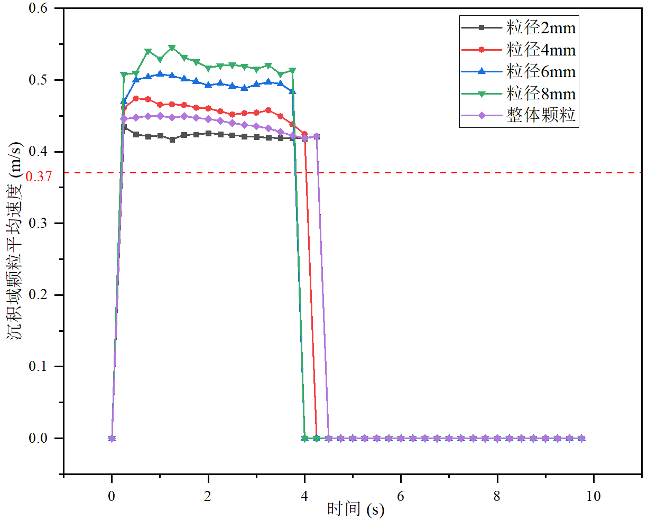
\includegraphics[width=0.48\textwidth]{figure/Wax-mean-velocity-Vin-dot37mpersec.png}
	}
	\subfloat[$V_{\mathrm{in}}=0.59\mathrm{m/s}$]{%
	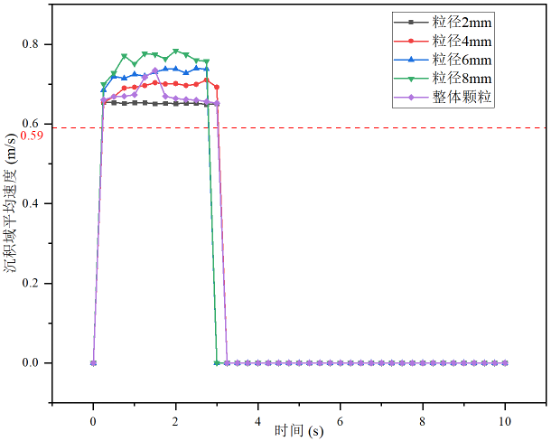
\includegraphics[width=0.48\textwidth]{figure/Wax-mean-velocity-Vin-dot59mpersec.png}
	}
	\caption{蜡垢颗粒在沉积域运移平均速度演化}
	\label{fig:Wax_velocity_particle_size}
\end{figure}

\subsection{井斜对蜡垢颗粒运移规律的影响}
本节改变井筒倾角，探究其对井筒环形空间内蜡垢颗粒运移的影响。选取井斜$\theta_c = 0^\circ$、45°、90°，洗井液入口流速为0.59m/s，粘度取$1.7\mathrm{mPa\cdot s}$，蜡垢颗粒粒径取2mm、4mm、6mm、8mm四种。图\ref{fig:wax_velocity_3angles}(a)描述了环空流体流速0.59m/s时0°井筒内不同粒径蜡垢颗粒在沉积域的平均速度变化情况：随着蜡垢颗粒粒径增大，其运移速度也增大，且均高于环空流体流速；在环空流体流速0.59m/s条件下，蜡垢颗粒在2.5s后到达压力出口。与45°井筒倾角工况相比，0°倾角井筒内蜡垢颗粒的最大运移速度更高，但其达到最大运移速度的时间长于45°井筒倾角工况。图\ref{fig:wax_velocity_3angles}(b)描述了环空流体流速0.59m/s时90°井筒内不同粒径蜡垢颗粒在沉积域的平均速度变化情况：随着蜡垢颗粒粒径增大，其运移速度反而减小，且均低于环空流体流速，可见摩擦力作用会导致蜡垢颗粒的运移速度下降；在环空流体流速0.59m/s条件下，蜡垢颗粒在4s后到达压力出口。与0°、45°井筒倾角工况相比，90°倾角井筒内蜡垢颗粒的最大运移速度明显下降，到达压力出口的时间变长，运移效率降低。


\begin{figure}[htbp]
	\centering
	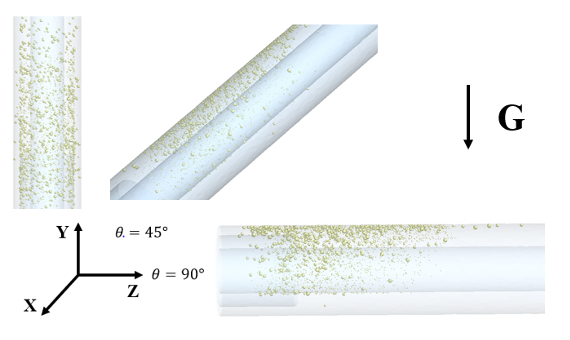
\includegraphics[width=0.7\textwidth]{figure/wax-distribution-3angles.png}
	\caption{不同井斜下蜡垢颗粒井筒内运移分布图}
\label{fig:wax_distribution_3angles}
\end{figure}


\begin{figure}[htbp]
	\centering
	\subfloat[$\theta=0^\circ$]{%
	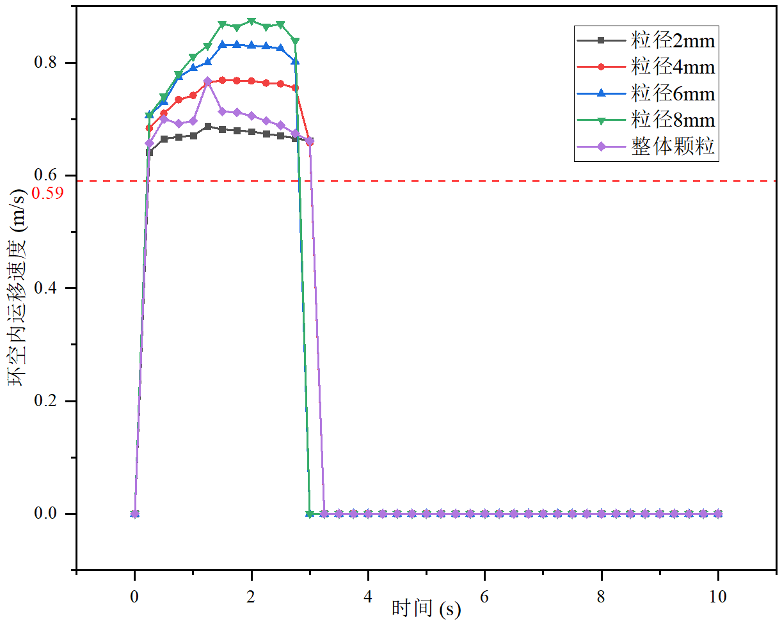
\includegraphics[width=0.48\textwidth]{figure/Wax-mean-velocity-Vin-dot59mpersec-theta-0.png}
	}
	\subfloat[$\theta=90^\circ$]{%
	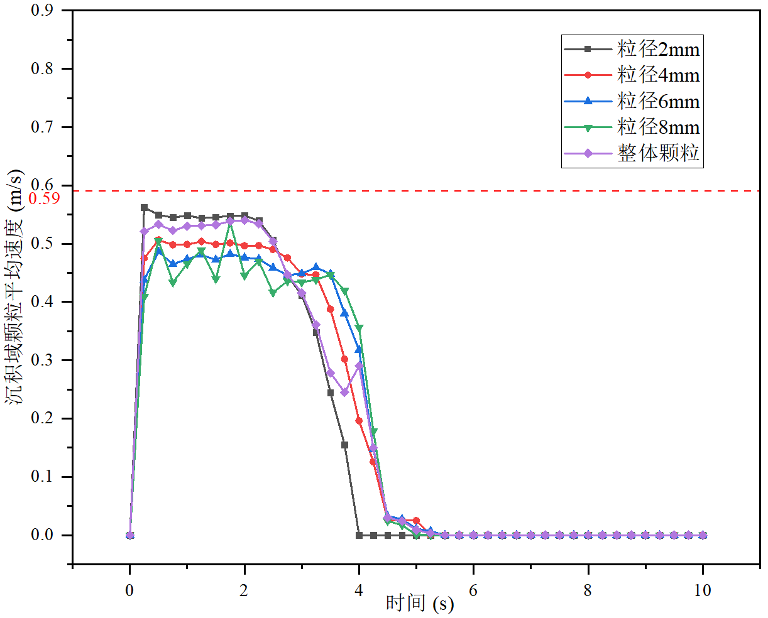
\includegraphics[width=0.48\textwidth]{figure/Wax-mean-velocity-Vin-dot59mpersec-theta-90.png}
	}
	\caption{井斜对蜡垢颗粒在沉积域运移平均速度演化的影响}
	\label{fig:wax_velocity_3angles}
\end{figure}

通过这些仿真发现，蜡垢颗粒的运移规律跟颗粒大小有关，在0°与45°井斜条件下，蜡垢颗粒的粒径越大，其运移速度越大。90°井斜条件下，蜡垢颗粒越小，其运移速度越大。随着井斜角度增加，蜡垢颗粒的运移速度也逐渐减小。 在各个井段并未发生蜡垢沉积现象。

\section{本章小结}

本章针对修井及洗井作业中砂砾、铁屑、结垢物（钡锶垢）和蜡质四类典型颗粒物在井筒内的运移及分布问题，基于流体动力学与颗粒动力学理论，建立了 EDEM--Fluent 双向耦合的液固两相流数值模拟方法，并以洗井液流速 $v_{\mathrm{in}}$、粘度 $\mu$ 和井斜角 $\theta$ 为核心控制变量，系统研究了四类颗粒在井筒环空内的运移轨迹、沉积速率及空间分布特征，主要结论如下：

（1）建立了井筒环空颗粒运移的 EDEM--Fluent 耦合仿真方法。颗粒相采用 Hertz--Mindlin 接触模型描述颗粒间以及颗粒与壁面间的接触、碰撞与摩擦作用，对含湿、存在液桥力的工况可采用 Hertz--Mindlin with JKR 接触模型；液固相间作用采用 Gidaspow 曳力模型，并计入 Saffman 剪切升力与 Magnus 旋转升力；液相采用 N--S 方程与标准 $k-\epsilon$ 湍流模型求解（部分工况采用 $SST\ k-\omega$ 模型），通过耦合接口实现颗粒运动与流场动量的双向传递。计算模型取长 $1.5$ m 的环空管段，模拟 $\phi 88.9$ mm 钻杆与 $\phi 244.475$ mm（$9$-5/8\inch）、$\phi 177.8$ mm（$7$\inch）井筒的组合工况，井斜角取 $0^\circ$、$45^\circ$、$90^\circ$，洗井液流速取 $0.17\sim0.69$ m/s，粘度取 $1.0\sim5.0\ \mathrm{mPa}\cdot\mathrm{s}$。

（2）基于现场砂样粒度分级统计结果（中砂 35.29\%、细砂 47.15\%、极细砂 13.99\%）建立了 9.9 万个不同粒径砂砾颗粒的仿真模型，获得了环空内砂砾的沉降与分布规律。钻杆静止时环空内砂砾质量在约 30 s 后趋于稳定，稳定沉积量平均约 $63.294$ kg；由于环空上部为流体高速区、下部为低速区，砂砾受重力作用大量沉降于环空下部低速区并形成砂床，砂砾床主要沉积在水平段，井斜角增大后井斜段内砂砾体积分数明显减小。随洗井液流速由 $0.17$ m/s 增至 $0.69$ m/s，砂床最高点（b 点）高度由 $68$ mm 降至 $32$ mm，且砂砾体积分数减小、砂砾流速增大，表明增大排量可增强流体携砂能力、降低砂堵风险；随洗井液粘度由 $1.0\ \mathrm{mPa}\cdot\mathrm{s}$ 增至 $5.0\ \mathrm{mPa}\cdot\mathrm{s}$，砂床最高点高度由 $77.5$ mm 降至 $25$ mm，但砂砾流速呈减小趋势，即增大粘度在提高携砂能力的同时会降低环空流体的流动性、延长砂砾上返时间。因此，工程上减小砂堵风险应以增大冲砂排量为主要手段，以适度提高洗井液粘度为辅。

（3）明确了颗粒在工具与井筒环空内沉积的“危险位置”。以外部功能单元最多、结构最复杂的“四合一”工具扶正器与强磁部位和 $7$\inch 井筒构成的环空为对象，在环空流速 $0.37$、$0.59$ m/s 下开展仿真，结果表明部分砂砾会因重力作用在工具前端产生堆积，并在强磁部件的凹槽内少量滞留；环空流速增大后颗粒的轴向位移与运移效率明显提高。工具的导流结构可引导砂砾随流运移，与增大冲砂排量相配合能够有效降低砂堵概率，为工具安全作业提供保障。

（4）揭示了铁屑颗粒“粘度弱敏感、流速强敏感、井斜角决定性”的运移规律。以井下封隔器套铣作业返出碎屑中的丝状铁屑（密度 $7800$ kg/m$^{3}$）为典型建模对象：颗粒在沉积域中的平均轴向速度始终小于来流平均速度，表明井壁摩擦对颗粒运移具有显著阻滞作用，随时间推移运移速度逐渐趋于稳定，颗粒运移达到动态平衡状态；粘度由 $1.0\ \mathrm{mPa}\cdot\mathrm{s}$ 增至 $1.7\ \mathrm{mPa}\cdot\mathrm{s}$（增至 $1.7$ 倍）时，沉积域内颗粒的平均运移速度仅增至 $1.04$ 倍，说明洗井液粘度对铁屑运移的影响十分有限；流速由 $0.17$ m/s 增至 $0.27$ m/s 时，颗粒的轴向位移与瞬时速度大幅提高，颗粒床的形成受到抑制，说明流速是铁屑运移最敏感的控制因素；井斜角的影响最为显著，直井（$\theta=0^\circ$）中流体拖曳力不足以克服重力，铁屑不能上返、必然下落至井底；$45^\circ$ 斜井中铁屑床堆积在靠近颗粒工厂一侧的底部井壁，出口附近几乎没有颗粒；水平井（$\theta=90^\circ$）中颗粒床迁移距离更远、聚集度更低、出口处颗粒数量更多，但移动铁屑床的平均运移速度仅约为环空平均流速的一半。据此推测存在临界井斜角 $\theta_c<45^\circ$：当 $\theta<\theta_c$ 时铁屑一致下落至井底形成堆积，当 $\theta>\theta_c$ 时铁屑在井壁堆积。上述结论可推广至片状、块状等高密度金属屑。可见在直井与小斜度井中，铁屑难以通过常规洗井液循环排出井筒，必须依靠具备\textbf{吸附}、\textbf{过滤}功能的\textbf{专用清洁工具}。

（5）阐明了结垢物（钡锶垢）颗粒的运移与沉积特征。以密度 $4336$ kg/m$^{3}$、特征长度分别约为 $10$ mm 和 $4$ mm 的两种钡锶垢颗粒为对象：随洗井液流速由 $0.37$ m/s 增至 $0.59$ m/s，垢颗粒的运移速度与轴向位移均增大；但在 $0.59$ m/s 时，三种井斜工况下的大颗粒垢均发生沉积，$0^\circ$ 井斜沉积于井底，$45^\circ$ 井斜先沉积于井壁继而向井底滑移，$90^\circ$ 井斜沉积于井壁；小颗粒垢的运移速度远低于环空流体流速（$0.37$ m/s 时约为 $0.05$ m/s、$0.59$ m/s 时约为 $0.25$ m/s），且随井斜角增大而减小；$45^\circ$ 与 $90^\circ$ 井斜下大小垢颗粒均会发生沉积。因此洗井作业时应重点清洗斜井段与水平井段，清除大块钡锶垢需要更高排量的水泵。

（6）明确了蜡垢颗粒的运移规律。蜡垢密度（$800$ kg/m$^{3}$）低于洗井液密度，在各计算工况下均未发生沉积。洗井液流速由 $0.37$ m/s 增至 $0.59$ m/s 时，颗粒运移速度增大，到达压力出口的时间由约 $4$ s 缩短至约 $2.5$ s；粒径与运移速度的关系随井斜角发生反转，$0^\circ$ 与 $45^\circ$ 井斜条件下粒径越大运移速度越大，$90^\circ$ 井斜条件下因井壁摩擦作用粒径越大运移速度反而越小；总体而言，随井斜角度增加蜡垢颗粒的运移速度逐渐减小。可见提高环空流速是改善蜡垢携带效果的有效途径。

需要指出的是，上述四类颗粒的仿真均在同心环空、光滑管壁、颗粒形状简化的条件下完成，未计入偏心环空、颗粒团聚、颗粒与工具全尺寸结构的相互作用以及地层非稳态出砂供给等因素，因此所得定量结果（如环空内沉积砂砾质量、砂床最高点高度、颗粒运移速度等）反映的是各工况下颗粒运移的规律性趋势，尚需通过室内物理模拟实验进一步检验，并逐步推广至偏心环空和更接近现场的多因素耦合工况。

综合本章研究可以看出，环空流体流速对砂砾、铁屑、钡锶垢和蜡质运移的控制作用最强，洗井液粘度的影响次之且对铁屑等高密度金属屑十分有限，而井斜角往往决定颗粒能否被携带出井筒；四类颗粒均倾向于在环空下部低速区或井壁处富集并形成颗粒床，仅依靠常规洗井液循环无法解决连续砂床、铁屑和顽固垢层在井筒内的残留问题。这既揭示了井筒清洁作业中砂堵、卡钻及工具失效风险的来源，也为后续开展室内颗粒运移实验、明确影响运移效果的主控因素，进而开发高效井筒清洁工具提供了理论依据。
